\problemname{Studschiffret}
\noindent
Fretchif has invented a revolutionary cipher that nobody will be able to crack!
Here is how it works: You choose a string to encrypt and two integers $N$ and $M$.
Then you draw a grid with $N$ rows and $M$ columns.
Next, you start writing out the string you are encrypting, one letter at a time, diagonally
downward to the right from the top-left corner. If we number the columns from
left to right $1$ to $M$, and the rows from top to bottom $1$ to $N$, then
the first letter ends up at position $(1,1)$, the second at $(2,2)$, the third at $(3,3)$,
and so on. When you reach one of the grid's walls, the ``letter ray''
bounces off the wall (see the sample explanation). If at any point you land on a
cell that already has a letter in it, you take the letter you were going to write and write
it in the next empty cell you reach instead. When all letters in the string to be
encrypted are used up, you read off the grid row by row, and that becomes the encrypted message.
\\ \\
Given a message that Fretchif encrypted with the bounce cipher,
and given the size of the grid that was used, print the original message.
\\ \\
Note that some messages cannot be encrypted with certain grid sizes,
since it is possible that you never reach any new empty cell but still
have letters left to place. Here, however, it is guaranteed that this
did not happen when Fretchif encrypted the string.

\section*{Explanation of Sample}
Say the string we want to encrypt is \texttt{ABCDEFGHIKLMNOPQRST}, and the grid has size $6 \times 13$.
Here is what the grid looks like at various points during the encryption: \hspace{25cm}
\begin{figure}[!h]
  \centering
      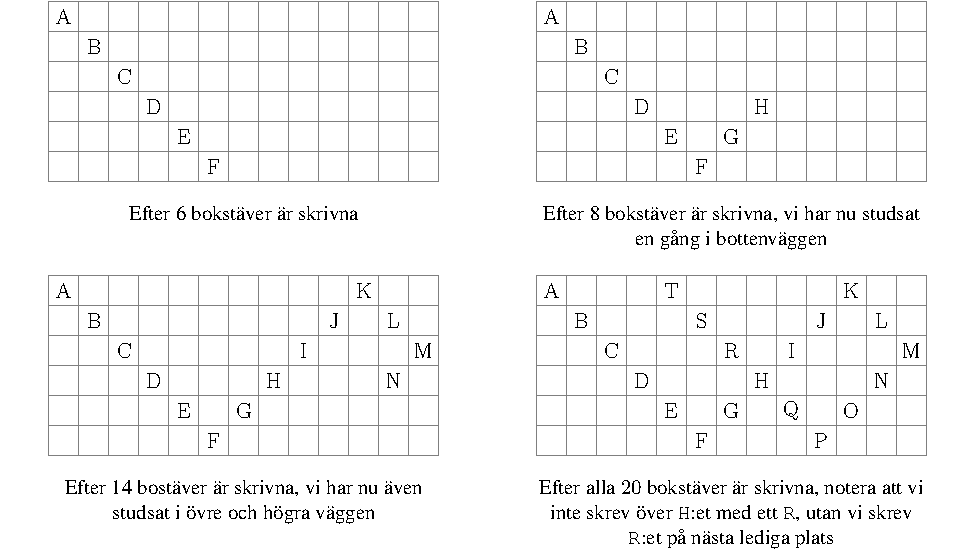
\includegraphics[width=1\textwidth]{grids.pdf}
\end{figure}

In this example, the encrypted message is thus \texttt{ATKBSJLCRIMDHNEGQOFP}.
Sample 2 is to decode \texttt{ATKBSJLCRIMDHNEGQOFP}, which decodes to \texttt{ABCDEFGHIKLMNOPQRST}.

\section*{Input}
The first line contains two integers $2 \leq N \leq 20$ and $2 \leq M \leq 20$, the number of rows and columns in the grid.
The second line contains a string of $K$ letters ($1 \leq K \leq 30$), the encrypted message. The message consists only of the letters \texttt{A} to \texttt{Z} and all letters are uppercase.
It is guaranteed that there is a possible original string that produces this ciphertext.

\section*{Output}
The program should print a single line with a string: the original message, as it looked before it was encrypted.

\section*{Scoring}
\noindent
\begin{tabular}{| l | l | p{12cm} |}
  \hline
  \textbf{Group} & \textbf{Points} & \textbf{Constraints} \\ \hline
  $1$    & $20$       & $N=2$ and the letter ray never bounces off the right wall. \\ \hline
  $2$    & $40$       & The letter ray never bounces off the right wall. \\ \hline
  $3$    & $40$       & No additional constraints. \\ \hline
\end{tabular}
